% Organization:
%% Define new commands, macros, etc. in macros.tex
%% Anything that you would put before \begin{document} should go in prelude.tex
%test
\documentclass[answers]{exam}
\usepackage{amsmath}
\usepackage{amsthm}
\usepackage{amsfonts}
\usepackage{amssymb}
\usepackage{mathrsfs}
\renewcommand{\qedsymbol}{$\blacksquare$}

\usepackage[shortlabels]{enumitem}
\setlist[itemize]{label=\textbullet}


\usepackage[french]{babel}
\usepackage[utf8x]{inputenc}
\usepackage[T1]{fontenc}

\usepackage{booktabs}
\usepackage{todonotes}
%%% this part allows todo notes inside the solution boxes
\let\todox\todo
\renewcommand\todo[1]{\todox[inline]{#1}}
%%%%
\usepackage{float}

\usepackage{graphicx}

\newcommand{\imagefloat}[2]{
	\begin{figure}[H]
    \centering
    \includegraphics[width= #2 \textwidth]{#1}
    \end{figure}
    }
    
\usepackage{hyperref}

\author{2ème bachelier bioingénieur}

\title{Questions de l'examen théorique de la partie électricité du cours [ELEC-H201]\\ donné par Johan GYSELINCK}

\pagestyle{headandfoot}
\firstpageheader{}{}{\tiny{Dernière modification: le \ddmmyyyydate \today \ à \currenttime }}

\begin{document}

%% \union - Example: \union{j \in J}{A_j}
\newcommand{\union}[2]{\underset{#1}\bigcup #2}

%% \inter - like \union, but with \bigcap
\newcommand{\inter}[2]{\underset{#1}\bigcap #2}

\newcommand\blfootnote[1]{%
  \begingroup
  \renewcommand\thefootnote{}\footnote{#1}%
  \addtocounter{footnote}{-1}%
  \endgroup
}

\maketitle
\thispagestyle{headandfoot}


\begin{questions}
\question{L’équation ci-dessous contient un certain nombre d’erreurs. La corriger/compléter à 4 endroits.
\begin{equation*}
\underline{I}_s = \underline{I}_m + I_r = \frac{\underline{V}_s}{X_m} + \frac{V_s}{R_r + j X_d}
\end{equation*}
Dessiner le schéma équivalent qui y correspond. Indiquer tous les phaseurs et tous les paramètres.
}
\begin{solution}
\begin{equation*}
\underline{I}_s = \underline{I}_m + \underline{I}_r = \frac{\underline{V}_s}{j X_m} + \frac{\underline{V}_s}{R_r/g + j X_d}
\end{equation*}
\todo{A faire: dessiner le schema equivalent}
\end{solution}

\question{De quel type de force magnétique s’agit-il dans l’équation ci-dessous? Compléter/corriger celle-ci à 2 endroits sachant que la force provient d’un courant sinusoidal de pulsation $\omega$. Y indiquer la partie utile de la force (entre parenthèses).
\begin{equation*}
F = 2\ \frac{\hat{B}}{2 \mu_0} S_{fer} \left( \frac{1 + \cos \omega t}{2} \right)
\end{equation*}
}
\begin{solution}
 Il s'agit d'une force magnétique d'attraction.
\begin{equation*}
F = 2\ \frac{\hat{B}^2}{2 \mu_0} S_{fer} \left( \frac{1 + \cos 2 \omega t}{2} \right)
\end{equation*}

La partie utile dans la parenthèse est le "$\frac{1}{2}$".
\end{solution}

\question{Ajouter à l'équation ci-dessous une troisième expression du rendement d'un transformateur.
\begin{equation*}
\eta = \frac{P_2}{P_1} = \frac{ P_1 - P_{\text{pertes}}} {P_1}
\end{equation*}
De quel côté le transformateur est-il alimenté ? Expliciter le fonctionnement où le rendement est nul ?\\
Donner une valeur réaliste (au \% près) pour le rendement nominal d'un transformateur réel de très grande taille.
}
\begin{solution}
\begin{equation*}
\eta = \frac{P_2}{P_1} = \frac{ P_1 - P_{\text{pertes}}} {P_1} = \frac{P_2}{P_2+P_{pertes}}
\end{equation*}
La puissance va du primaire au secondaire. Il est donc alimenté au primaire (à confirmer ?).
Le rendement est nul lorsqu'aucune charge n'est connectée au secondaire.

Un transformateur réel de très grande taille (de 100 MVA ou plus par exemple) a généralement un rendement supérieur à 99\% (les pertes nominales sont inférieures à 1\%).
\end{solution}

\question{ Les véhicules routiers purement électriques ont à l'heure actuelle 2 inconvénient pratiques majeurs, à l'achat et pour l'utilisation, qui proviennent du moyen de stockage d'énergie. Discutez brièvement:
\begin{itemize}
\item à l'achat
\item pour l'utilisation
\end{itemize}
Quels sont les moyens de freinage ("verts" et "moins verts") que possède un tel véhicule ? Discutez brièvement:
\begin{itemize}
\item freinage "vert"
\item freinage "moins vert"
\end{itemize}
}
\begin{solution}
\begin{itemize}
\item A l'achat : le prix élevé
\item Pour l'utilisation:  l'autonomie est limitée,  présence d'une batterie qu'il faut recharger et qui peut être encombrante (les moteurs thermiques sont plus compacts et plus autonomes). %sous la figure 1.5 dans le syllabus
\end{itemize}

\begin{itemize}
\item Freinage vert:  freinage avec récupération: on fait fonctionner le moteur en génératrice pendant le temps du freinage et l'énergie électrique récupérée est renvoyée à la batterie pour la charger (juste avant 1.4 - électronique de puissance - dans le syllabus).
\item Freinage "moins vert" : freinage par frottement  $\Rightarrow$ énergie du freinage convertie en chaleur (perdue).
\end{itemize}

\end{solution}

\question{
Quels sont l'intérêt et la  nécessité d'utiliser plusieurs niveaux de tension dans les réseaux électriques AC (de 50 ou 60 Hz) ?
\begin{itemize}
\item l'avantage des hautes tensions
\item la nécessité des basses tensions
\end{itemize}
Ce changement de niveau de tension (et courant) est traditionnellement réalisé par des transformateurs. Quels sont leurs atouts (notamment par rapport à l'électronique de puissance que l'on pourrait également mettre en oeuvre à cet effet) ?
\begin{itemize}
\item la technologie
\item le rendement
\end{itemize}
}
\begin{solution}
\begin{itemize}
\item Hautes tensions : V élevé donc I peu élevé --> plus petit section de cuivre et donc moins cher
\item Basses tensions : 220V pour le domestique (basse pour une raison de sécurité)
\end{itemize}

\begin{itemize}
\item La technologie: transformateur : appareil permettant de transporter l'énergie magnétiquement
\item Le rendement: de 90 à 99\% (pour les plus gros)
\end{itemize}
Atouts par rapport à une autre technologie: pertes énergétiques minimum et rapport de tension peu variable. Les transformateurs sont aussi beaucoup plus fiables que l'électronique de puissance (ils ne tombent pas en panne contrairement à l'électronique) (et peut-être même plus avantageux en terme de longévité ?)
\end{solution}

\question{Quel type de moteur est très couramment utilisé dans les jouets à pile ou à batterie ? Quel est le premier soucis de fabrication pour ce type d'application ? Nommer deux aspects qui importent très peu (par rapport aux moteurs utilisés dans l'industrie).
\begin{itemize}
\item type de moteur
\item premier souci
\item important très peu
\end{itemize}
}
\begin{solution}
\begin{itemize}
\item Type : moteur à courant continu.
\item Premier soucis: présence de balais qui s'usent à la longue et peuvent produire des étincelles s'ils sont trop usés $\Rightarrow$ il faut le prendre en compte dans la fabrication du jouet .
\item Important très peu: la valeur de la tension utilisée est faible et le rendement est faible.
\end{itemize}

\end{solution}

\question{Quelle équivalence la figure ci-dessous illustre-t-elle ? Indiquer les 3 types de matériaux différents (4 fois ...... ).

Donner le nom précis et l'unité précise du paramètre B.

Comment appelle-t-on le produit $ni$ ? Quelle est son unité (en deux mots) ?

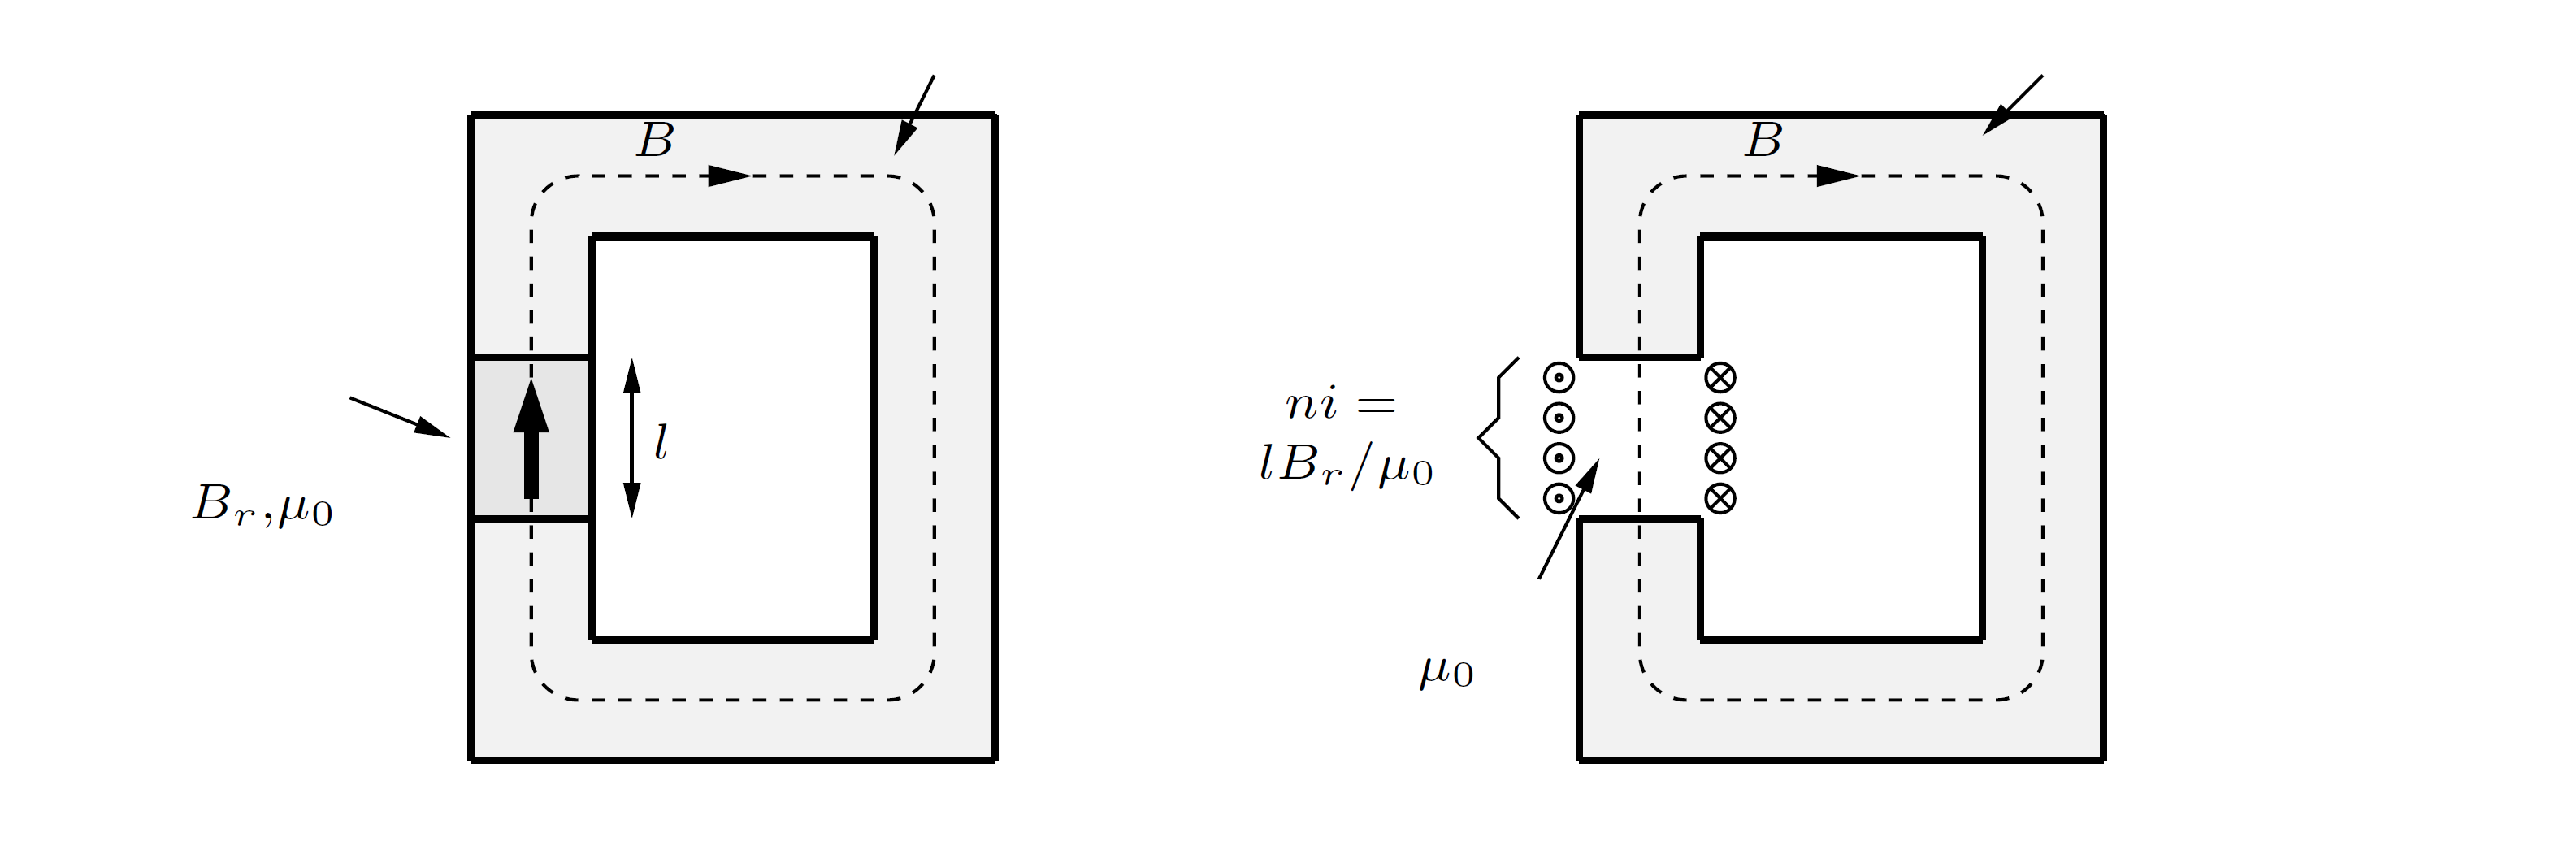
\includegraphics[width= 0.7 \textwidth]{./img/entrefer}
}
\begin{solution}
\begin{itemize}
\item L'équivalence entre circuit magnétique à aimant permanent et circuit magnétique à entrefer et bobines 
\item Matériaux non magnétiques, magnétiques (dur ), conducteur  ?? (dans le syllabus il a mis fer, entrefer et aimant permanant, je ne sais pas si c'est ça qu'il entend par "matériau")
\item B est l'induction ou la densité de flux, mesurée en Tesla (T)
\item Le produit ni est la force magnétomotrice, l'unité l'Ampère-tours.
\end{itemize}
\end{solution}
\question{ Donner trois avantages importants et l'inconvénient majeur de la traction électrique de véhicules routiers (par rapport à ceux à traction conventionnelle). 
}
\begin{solution}
\begin{itemize}
\item Vitesse des machines électriques peut être inversée et reglée dans une plage de vitesse importante sans boîte de vitesse
\item Rendement nominal des moteurs élec élevé (de 80 à 90\%, dépendant de la taille)
\item Moteurs électriques peu bruyant et pas polluants
\item Possibilité d'exploiter l'énergie de freinage en électrique
\item Moteurs à combustion plus compacts et ont une meilleure autonomie
\end{itemize}
\end{solution}
\question{ Compléter le tableau ci-dessous avec les noms des grandeurs manquantes et leur unité. Dessiner dans le plan B versus H la caractéristique d'un "matériau magnétique parfait". Quel en serait l'équivalent électrique ?

\begin{figure}[H]
\centering
\begin{tabular}{ll}
    \toprule
    Circuits électriques & Circuits magnétiques\\
    \midrule
    \midrule
    ...... & Flux magnétique (Wb)\\
    \midrule
    Tension (V) & ......\\
    \midrule
    Résistance ($\Omega$) & Réluctance (At/Wb)\\ 
    \midrule
    Conductivité (1/(m$\Omega$)) & ......\\
    \bottomrule
\end{tabular}
\end{figure}
}
\begin{solution}
\begin{figure}[H]
\centering
\begin{tabular}{ll}
    \toprule
    Circuits électriques & Circuits magnétiques\\
    \midrule
    \midrule
    Courant I (A) & Flux magnétique (Wb)\\
    \midrule
    Tension (V) & Force magnétomotrice $F = ni (A)$\\
    \midrule
    Résistance ($\Omega$) & Réluctance (At/Wb)\\ 
    \midrule
    Conductivité (1/(m$\Omega$)) & Perméabilité $µ = B/H (H/m)$\\
    \bottomrule
\end{tabular}
\end{figure}
\todo{Dessiner la caractéristique d'un "matériau magnétique parfait"}
\end{solution}

\question{En quoi les deux moteurs électriques montrés ci-dessous sont-ils particuliers ? Comment ceux-ci sont-ils alimentés ? De quel domaine d'application s'agit-il ?

De quels types (et sous-types) de machines électriques s'agit-il ? Voir les flèches indiquant des composants caractéristiques.

De quels composants s'agit-il dans les deux cas respectifs ? Compléter la figure par un mot pour chaque cas. Quel est le rôle primordial du composant indiqué dans la figure de gauche ?

\begin{minipage}{0.5\textwidth}
\centering
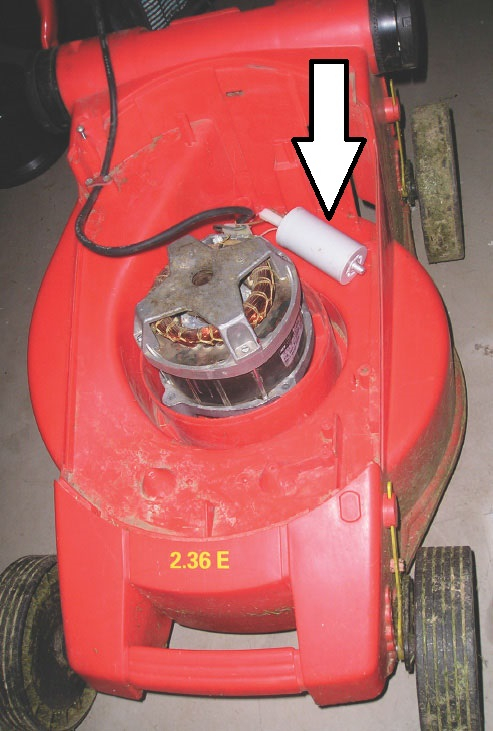
\includegraphics[width= 0.5 \textwidth]{./img/tondeuse}
\end{minipage}
\begin{minipage}{0.5\textwidth}
\centering
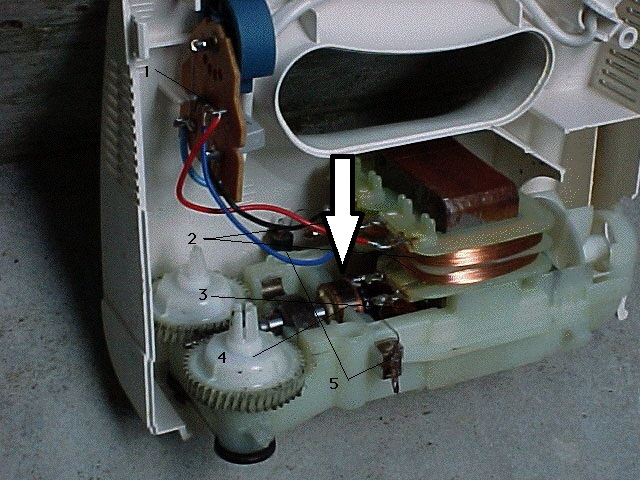
\includegraphics[width= 0.7 \textwidth]{./img/mixeur}
\end{minipage}
}
\begin{solution}
A gauche : moteur d'une tondeuse à gazon (moteur asynchrone alimenté en monophasé).\\
A droite : moteur universel de mixeur (moteur à courant continu alimenté en alternatif).\\
Domaine d'application : domestique.\\

Type de machine: machines tournantes

Composant indiqué :\\
A gauche : condensateur : rôle = compenser la perte de puissance réactive en en débitant.\\
A droite : ça ressemble au collecteur, qui est constitué des bagues et des balais. C'est une pièce essentielle des moteurs DC universels qui peut s'user ce qui est un désavantage  de ce type de moteur (pour la reconnaître: on voit qu'elle est un peu noire ce qui prouve l'usure des balais sur le collecteur).
\end{solution}

\question{ Pour chacune des 3 puissances actives et des 3 puissances réactives indiquées dans la figure ci-dessous, écrire une expression en exploitant les paramètres du schéma équivalent et les tensions et courants indiqués (en phaseur ou en valeur efficace). Pour les grandeurs secondaires accentuées, ne pas supprimer l'accent.

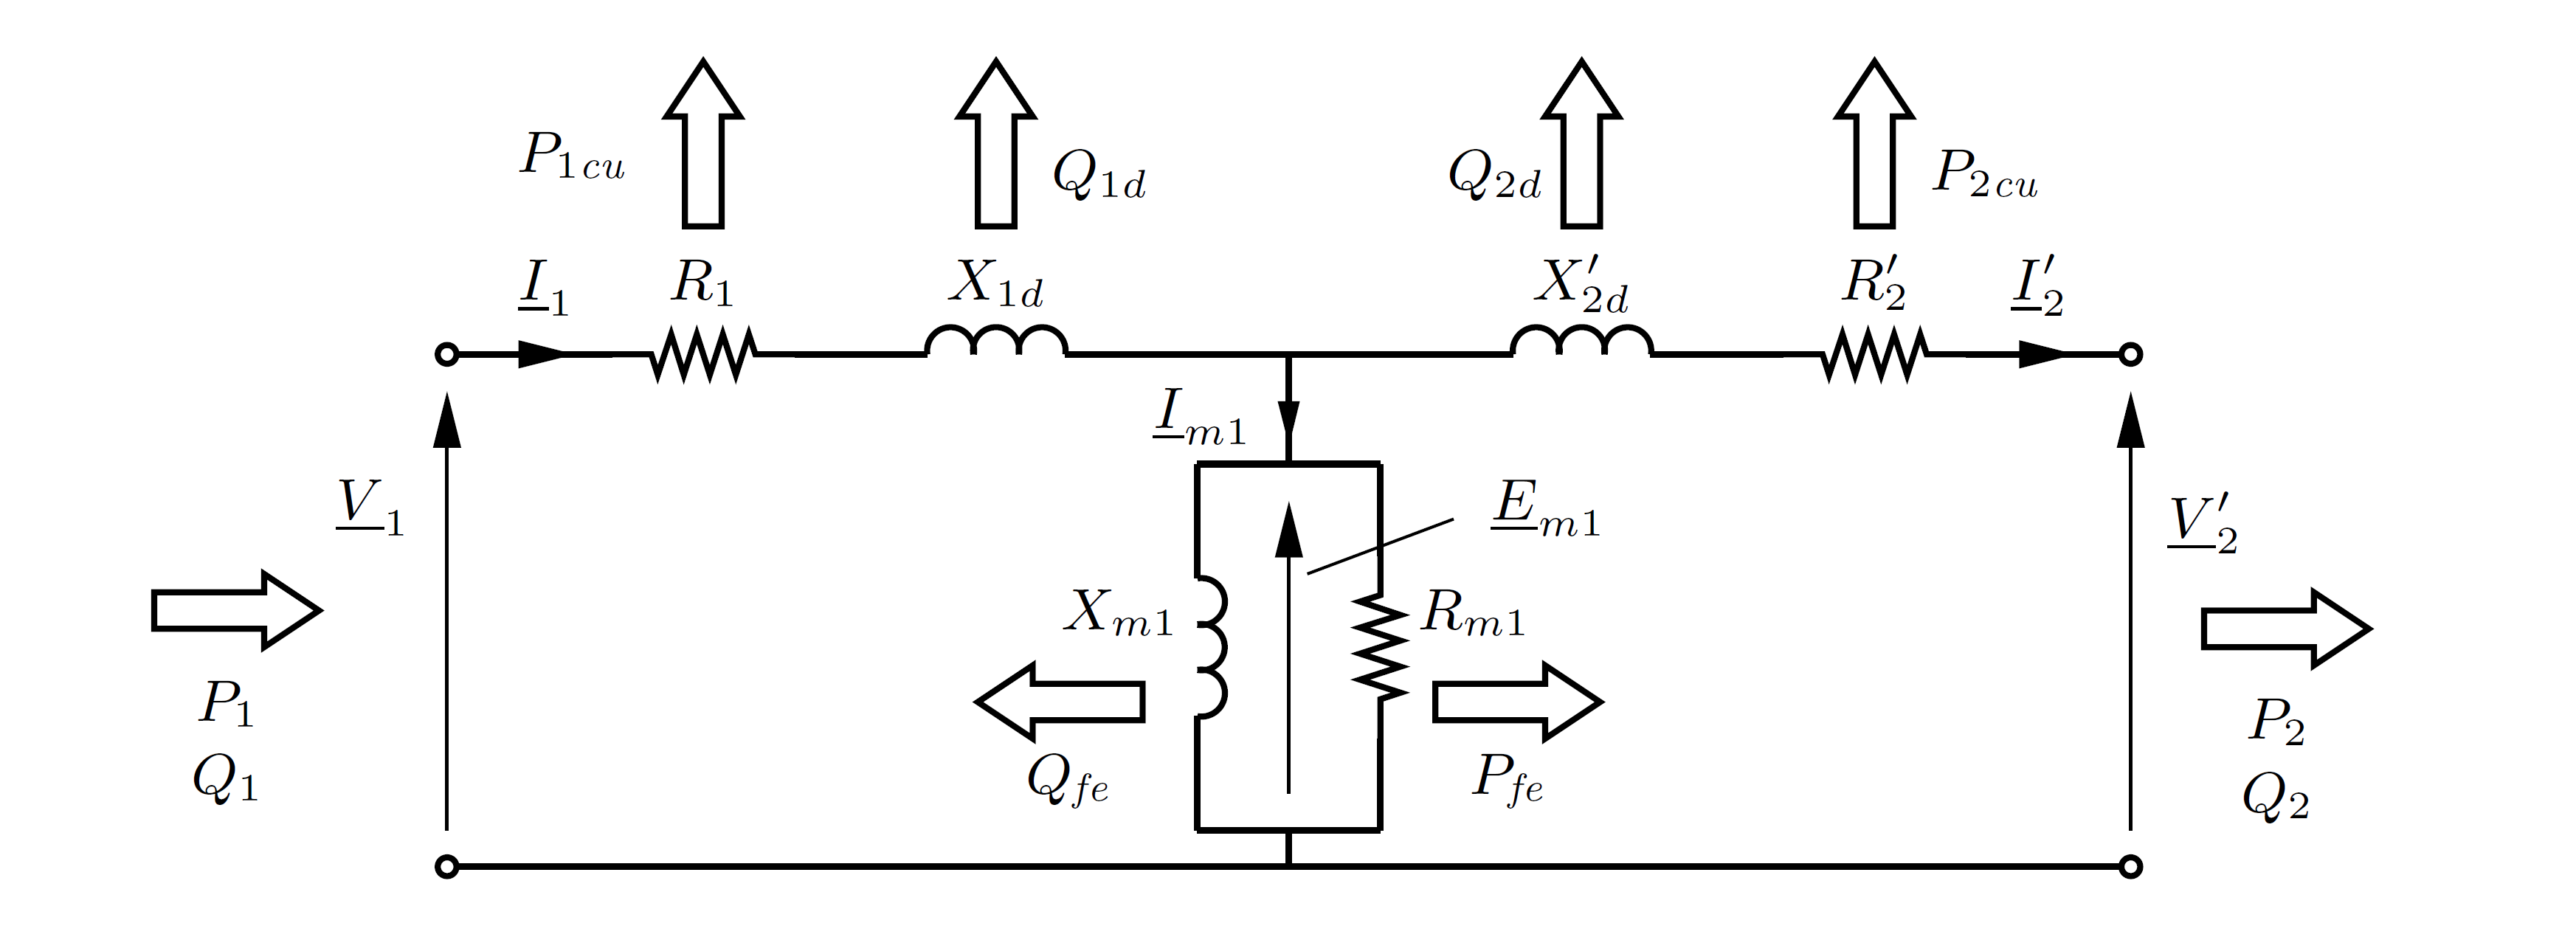
\includegraphics[width= 0.7 \textwidth]{./img/schema_eq}
}
\begin{solution}
\begin{align*}
P_{1cu} &= \underline{I}_1^2 R_1 & Q_{2d} &= X'_{2d} \underline{I}_2^{\prime2}\\
Q_{1d} &= \underline{I}_1^2 X_{1d} & P_{2cu} &= R'_2 \underline{I}_2^{\prime 2}\\
\end{align*}
\end{solution}

\question{Donner 2 filières en énergies renouvelables qui sont affectées par l'inconvénient de l'intermittence de la production. En donner une autre qui l'est beaucoup moins ou pas du tout.
\begin{itemize}
\item production intermittente (2)
\item production non ou peu intermittente (1)
\end{itemize}
}
\begin{solution}
\begin{itemize}
\item Photovoltaïque et éolien
\item Biomasse
\end{itemize}
\end{solution}

\question{ Soit le transformateur monophasé montré ci-dessous. Que vaut son rapport de transformation (symbole + expression générale + valeur) ?

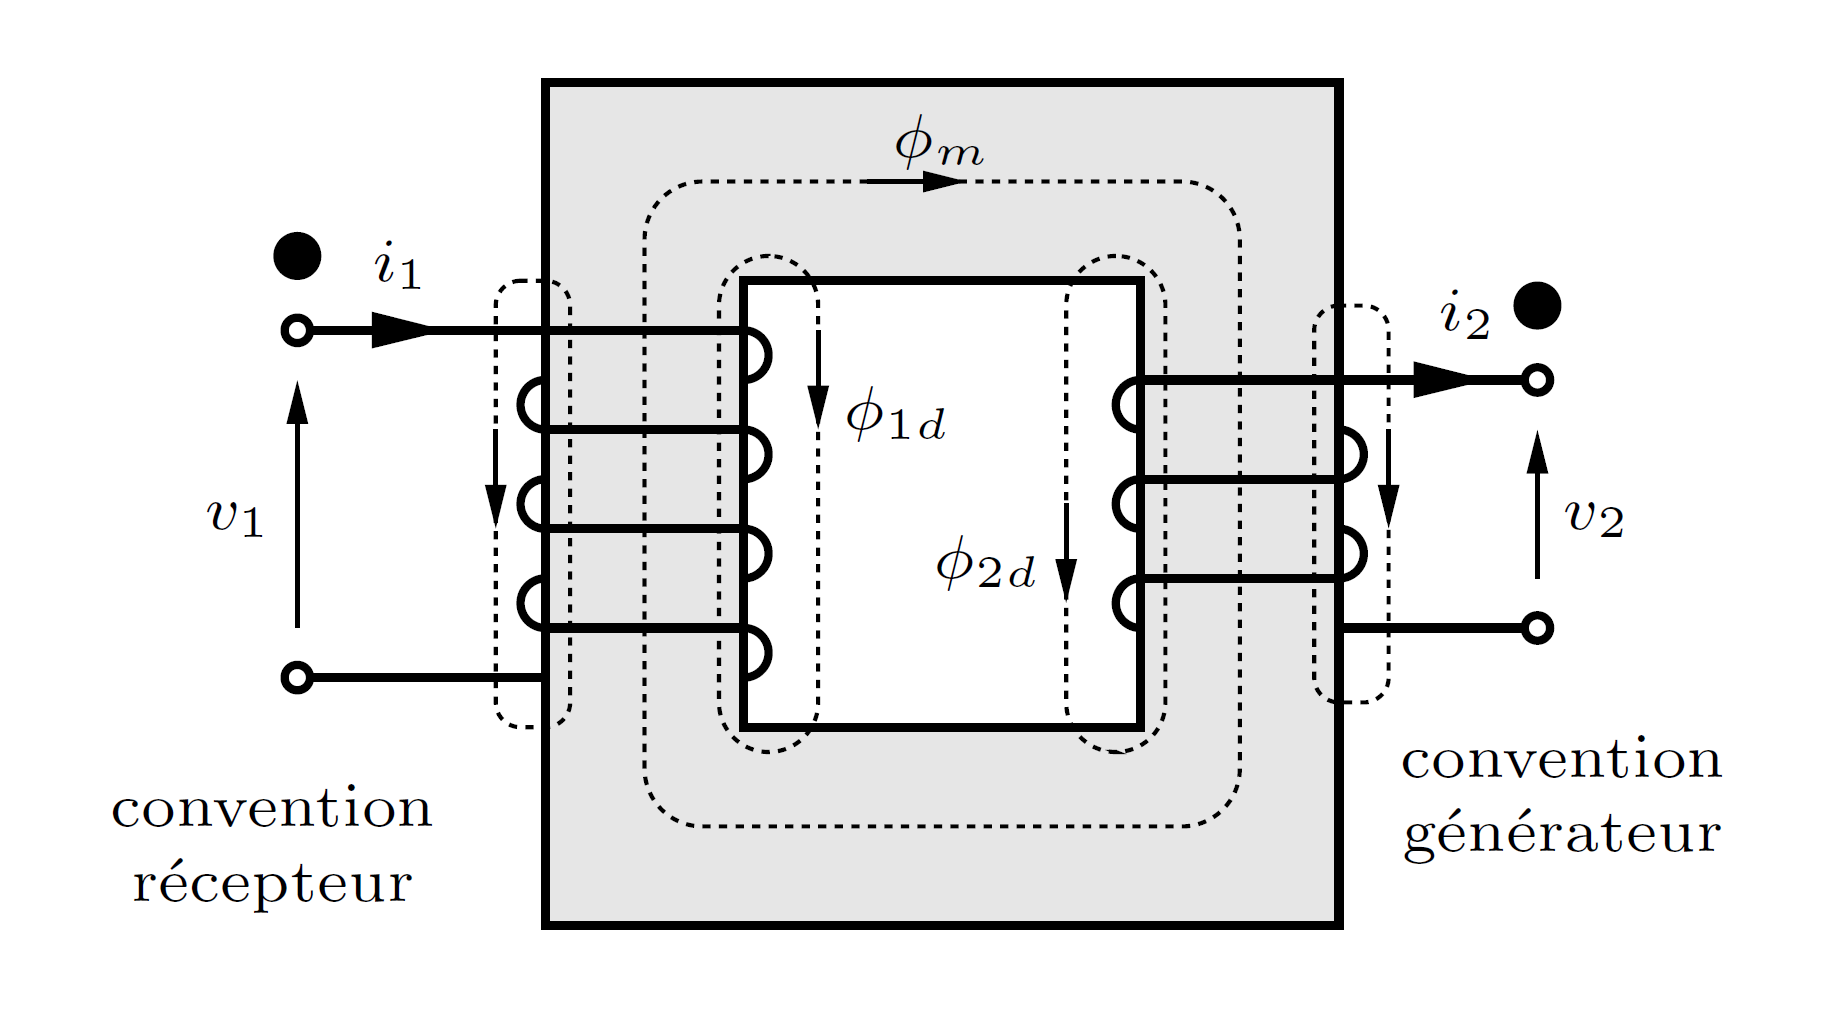
\includegraphics[width= 0.5 \textwidth]{./img/transformateur}

Donner l'équation qui relie les deux tensions instantanées en supposant que le transformateur est idéal. De même pour les deux courants instantanés. En déduire la conservation de la puissance instantanée. 
}
\begin{solution}
$a=\frac{N_1}{N_2}=\frac{4}{3}$\\
Si le transformateur est idéal, $\frac{v_1}{v_2}=a$ et $\frac{i_1}{i_2}=\frac{1}{a} \Rightarrow p_1 = p_2$
\end{solution}

\question{L'équation ci-dessous comprend 6 grandeurs ou paramètres primaires, ceux secondaires et le rapport de transformation a (au carré). Donner pour chaque grandeur/paramètre (p. ex. primaire) le nom précis et l'unité précise.
\begin{equation*}
\frac{R_1}{R_2} = \frac{\frac{\rho_1 N_1 l_1}{I_1 / J_1}}{\frac{\rho_2 N_2 l_2}{I_2 / J_2}} \approx \left( \frac{N_1}{N_2} \right)^2 = a^2
\end{equation*}

Donner et expliquer brièvement les quatre hypothèses/simplifications qui mènent à l'approximation proposée.
}
\begin{solution}
$\rho$ = résistivité en $\Omega m$ et on considère que c'est la même au primaire et au secondaire (1ère hypothèse).\\
$N$ = nombre de spires, et $\frac{N_1}{N_2} = a$ (définition de a).\\
$l_1=l_2$ (en $m$), longueur d'une spire (3ème hypothèse).\\
$J_1=J_2$ densité de courant en $A/m^2$ (4ème hypothèse).\\
On a aussi $\frac{I_2}{I_1} = a$, et on obtient donc le résultat attendu.
\end{solution}

\question{Ajouter à l'équation ci-dessous du rendement du transformateur (pour la puissance allant du primaire au secondaire) deux expressions en terme des pertes totales $P_{pertes}$ dans celui-ci.
\begin{equation*}
\eta = \frac{P_2}{P_1} = 
\end{equation*}

Quels sont les deux fonctionnements très particuliers qui donnent lieu à un rendement nul ?

De façon très générale, quelles sont les trois composantes de pertes énergétiques dans un transformateur ?
}
\begin{solution}
\begin{equation*}
\eta = \frac{P_2}{P_1} = \frac{P_1 - P_{pertes}}{P_1} = \frac{P_2}{P_2 + P_{pertes}}
\end{equation*}

Les deux fonctionnements particuliers :
A vide et en court-circuit


 Les 3 pertes :
 \begin{itemize}
\item pertes fer (hystérésis et courants de Foucault)
\item pertes cuivre (pertes joules)
\item flux de dispersion 
\end{itemize}
\end{solution}

\question{Dans les entraînements à machine asynchrone, un gradateur triphasé (voir la figure ci-dessous) peut être utilisé pour deux raisons. lesquelles ?

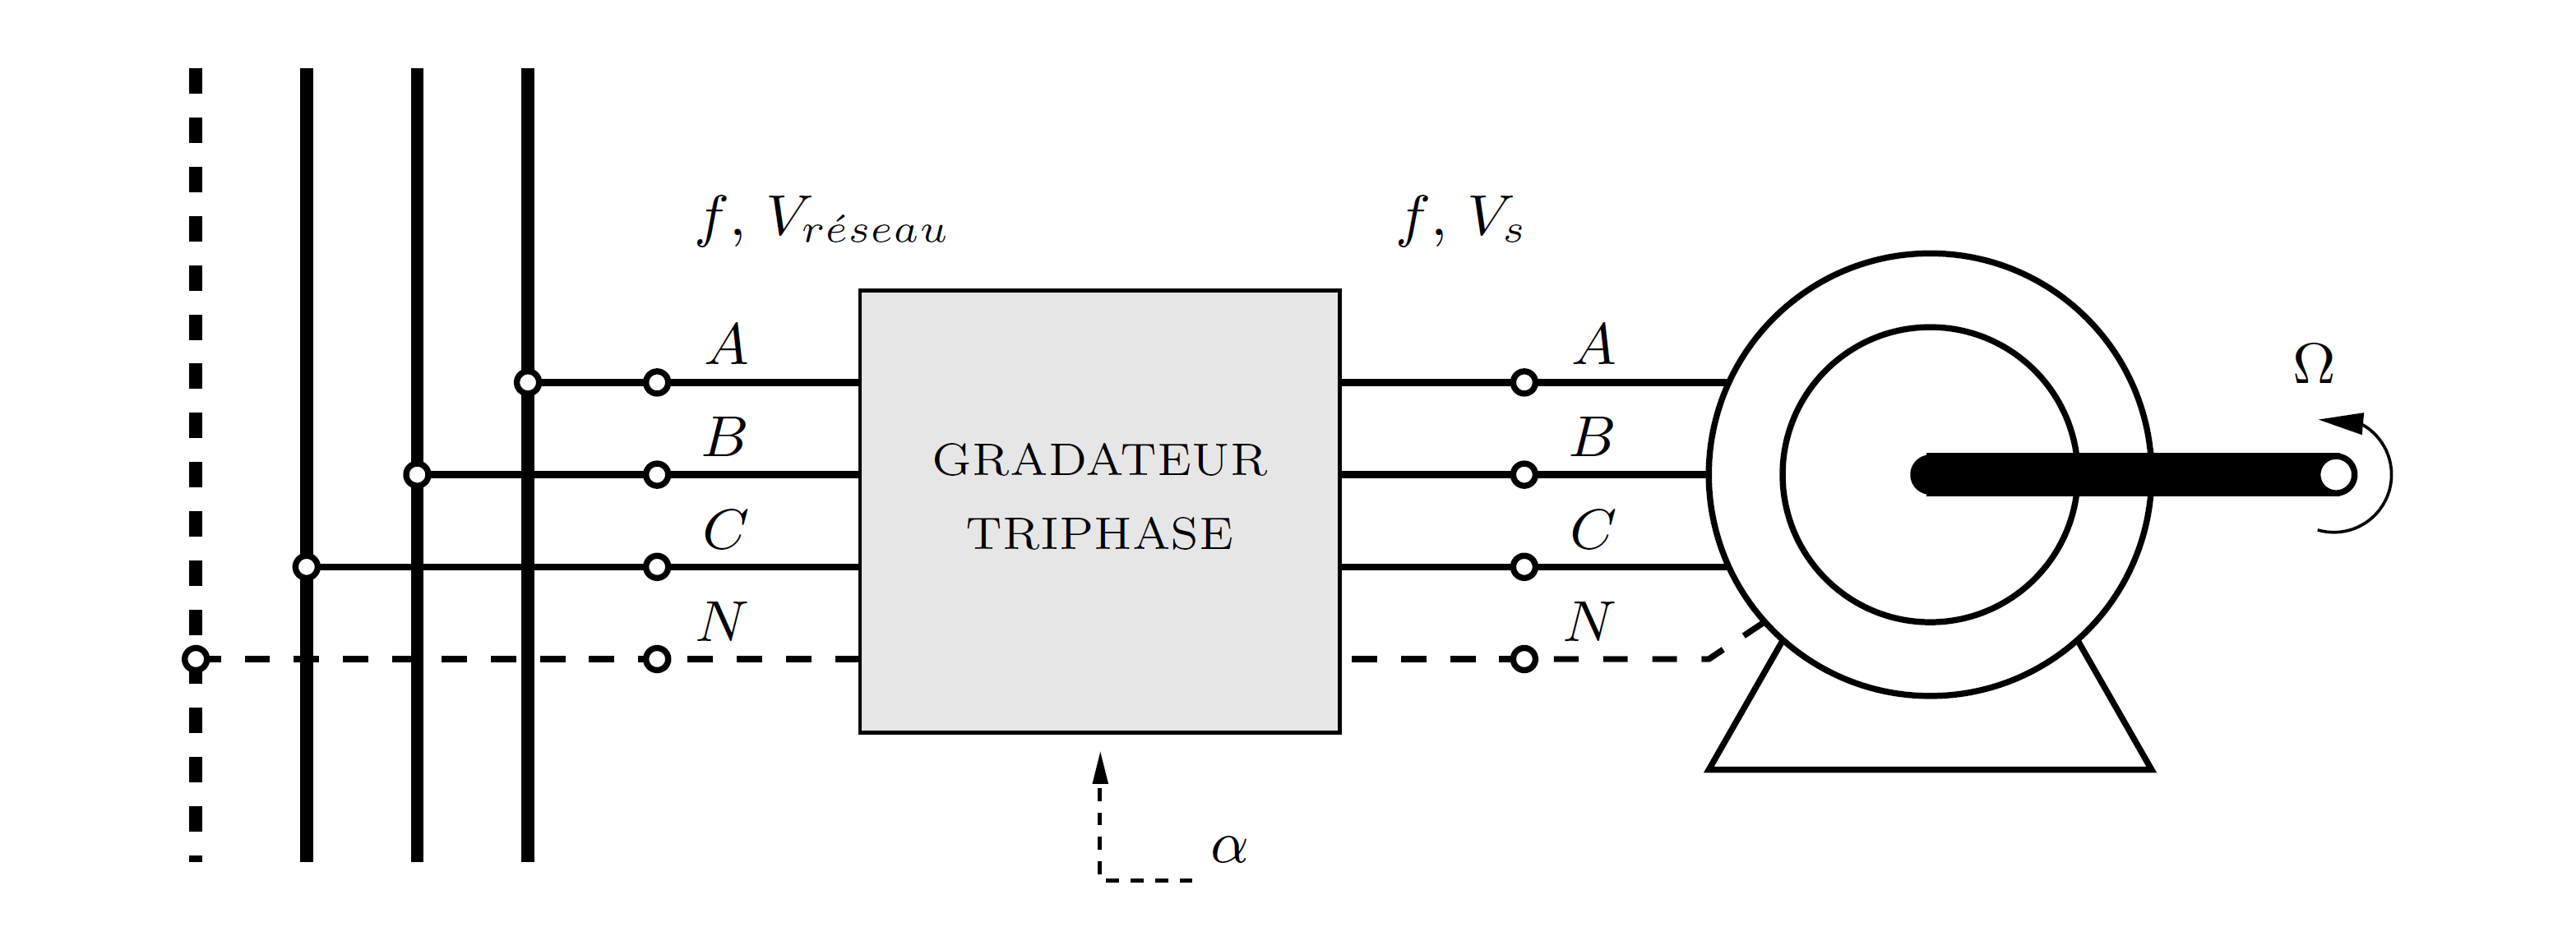
\includegraphics[width= 0.7 \textwidth]{./img/gradateur}

Quel type de conversion électronique de puissance le gradateur effectue-t-il . Que peut-on dire quant à la fréquence ? Quid de la tension de sortie (et sa composante fondamentale) ?

S'agit-il d'une machine à cage ou d'une machine à rotor bobiné ? Justifier.
}
\begin{solution}
Le gradateur va faire baisser l'amplitude du signal du coup la tension diminuera proportionnellement. La fréquence n'est pas modifiée mais le rendement diminue. Il s’agit d’un montage électronique de puissance très simple et peu coûteux.
C'est une machine à cage car les gradateurs sont peu coûteux et nécessitent une maintenance réduite.
\end{solution}

\question{Soit le transformateur monophasé montré ci-dessous. Que vaut son rapport de transformation (symbole + expression générale + valeur) ?

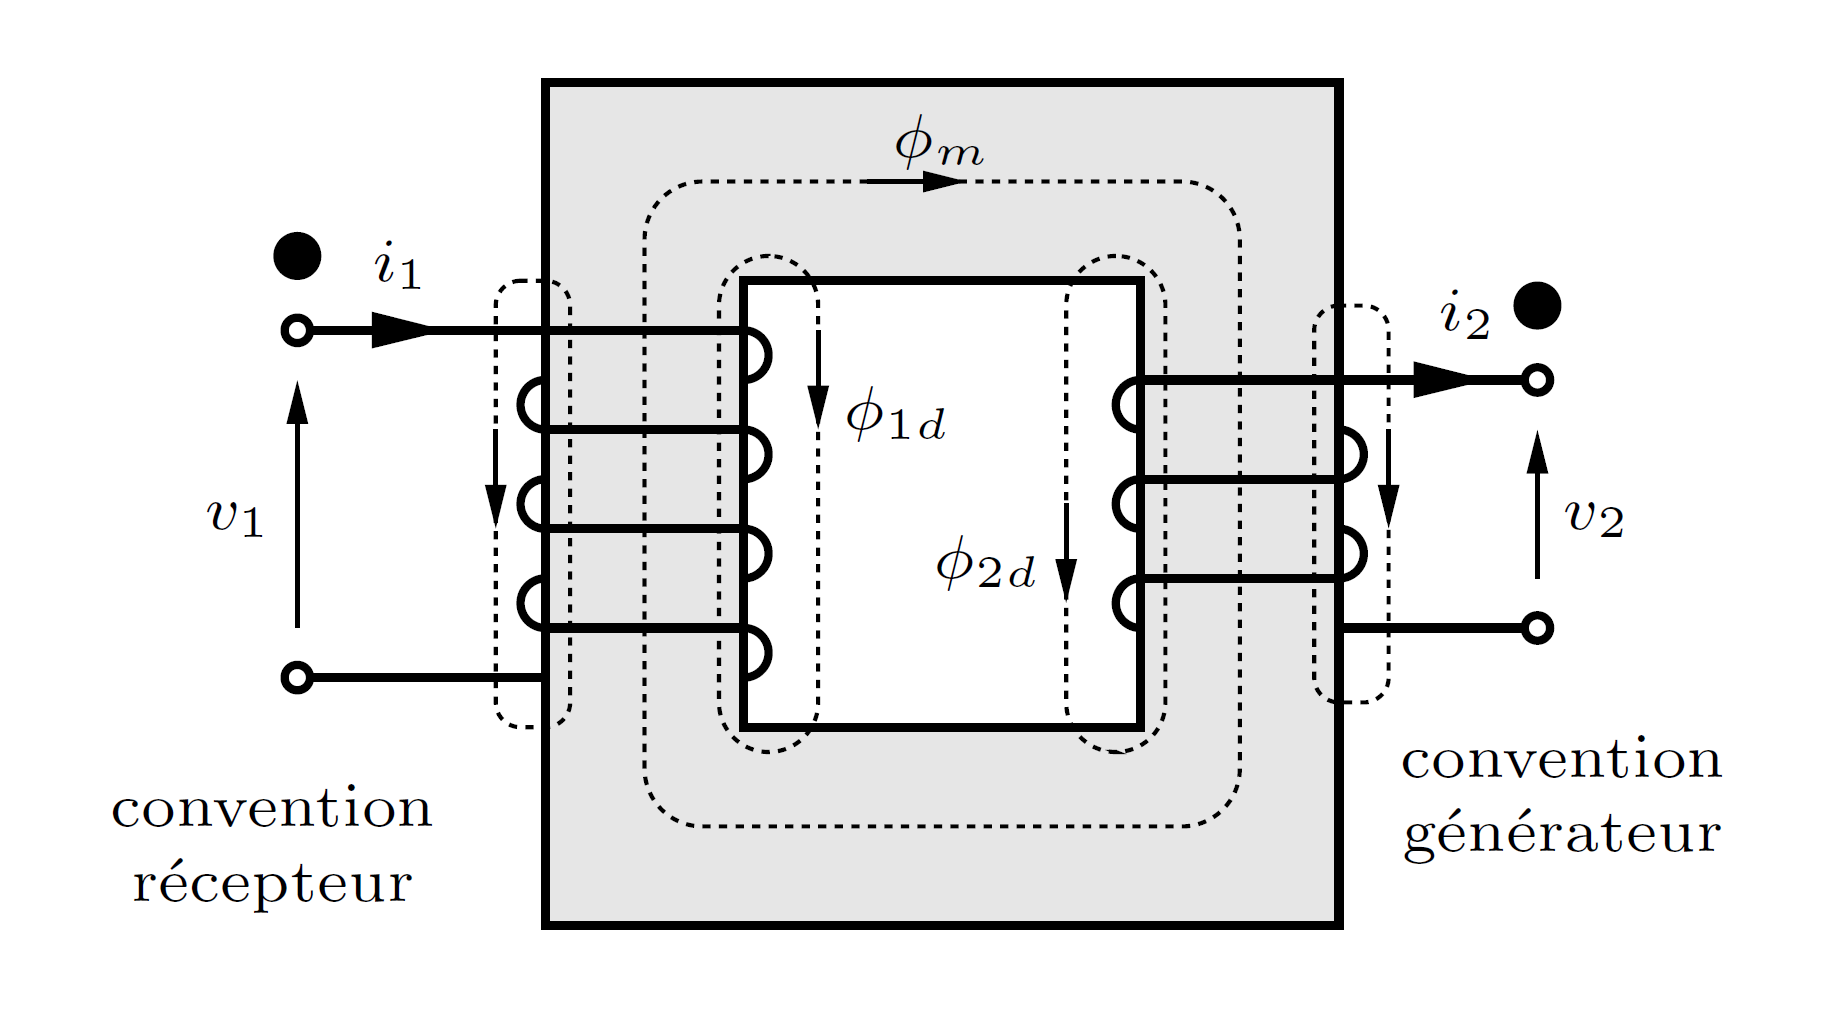
\includegraphics[width= 0.5 \textwidth]{./img/transformateur}

Nommer de façon précise les trois types de flux magnétique indiqués dans la figure.

Donner l'expression précise (avec symboles usuels) de la puissance instantanée absorbée par le primaire, ainsi que celle débitée par le secondaire, en exploitant les grandeurs indiquées dans la figure.

Donner les deux expressions correspondantes de puissance active (en utilisant les symboles et la notation usuels).
}
\begin{solution}
$\phi_{1d}$ = flux de dispersion au primaire.\\
$\phi_{2d}$ = flux de dispersion au secondaire.\\
$\phi_{m}$ = flux de magnétisation.\\

Puissance instantanée:\\
$p_1 = v_1 i_1$ et $p_2 = v_2 i_2$\\
Puissance active:\\
$P_1= V_1 I_1 \cos \phi_1$\\
$P_2= V_2 I_2 \cos \phi_2$\\
\end{solution}

\question{ A partir du schéma équivalent complet d'une machine asynchrone montré ci-dessous, dessiner le schéma simplifié à trois éléments (qui ne peut être simplifié davantage). Donner le nom précis et l'unité précise des 4 paramètres de ce schéma simplifié.

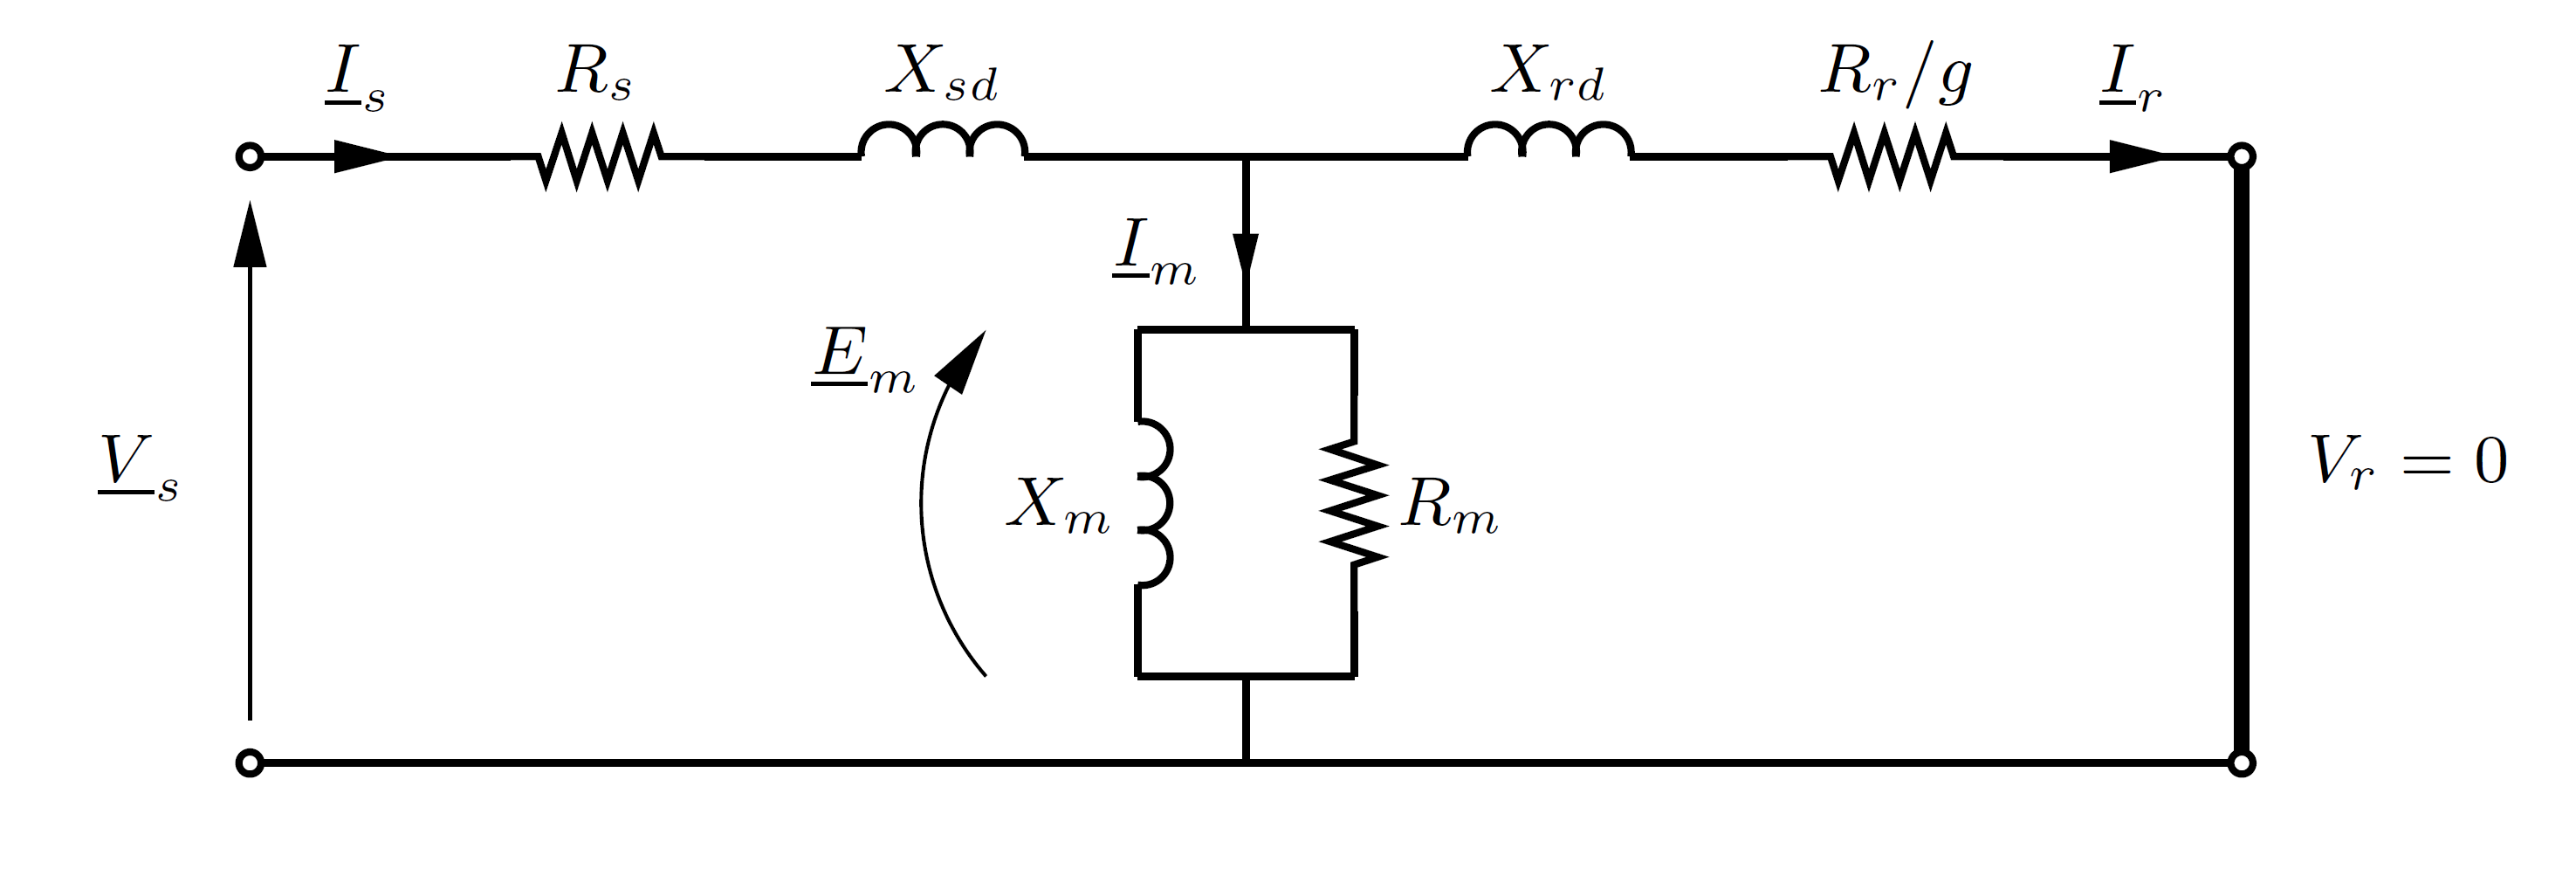
\includegraphics[width= 0.7 \textwidth]{./img/schema_compl}
}
\begin{solution}\\
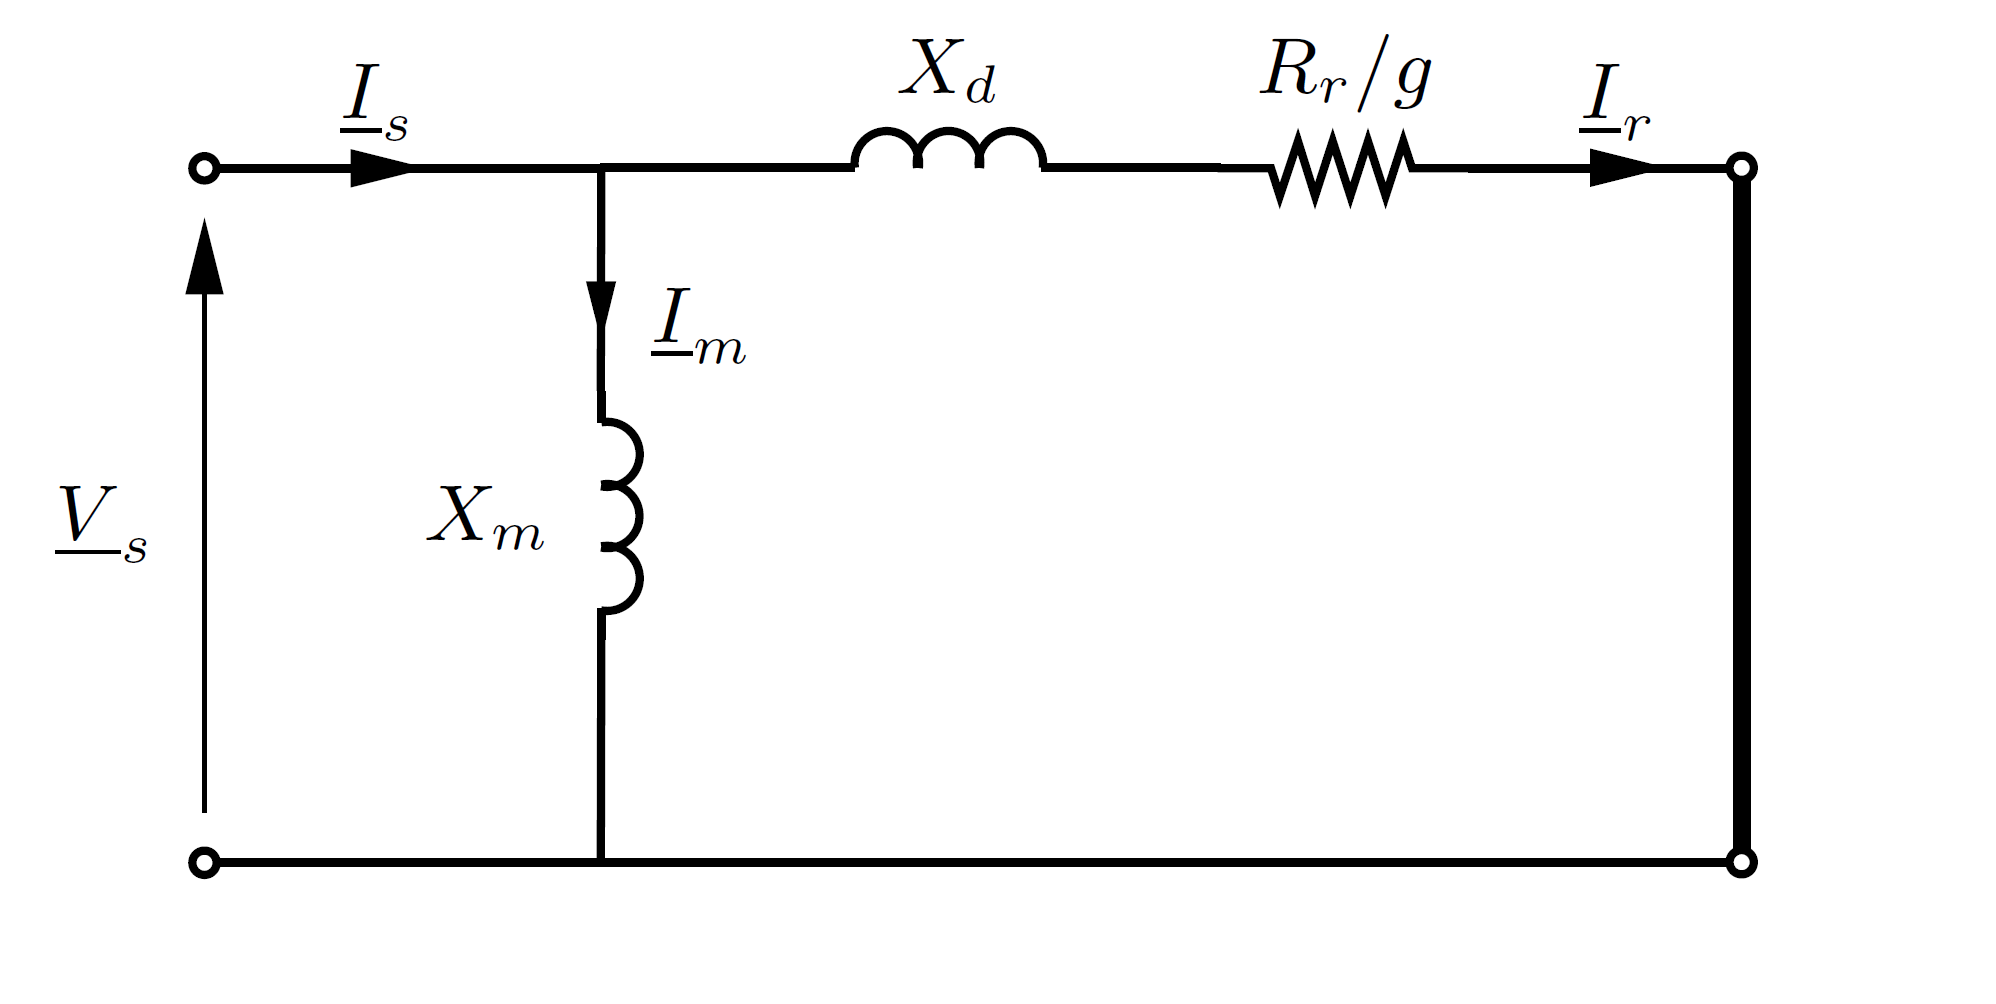
\includegraphics[width= 0.7 \textwidth]{./img/schema_simpl}


$V_s$ = tension d'alimentation (V)\\
$I_s$ = phaseur du courant circulant dans les phases de l'enroulement statorique (A)\\
$I_r$ = courant rotorique (A)\\
$I_m$ = courant de magnétisation (A)\\
\end{solution}

\question{Soit la figure ci-dessous qui a trait aux machines asynchrones. De quel composant ou partie de composant s'agit-il ?

Ce type de construction de machine est-il courant dans la pratique ? Justifier.

Quel est l'autre type de machine asynchrone ?

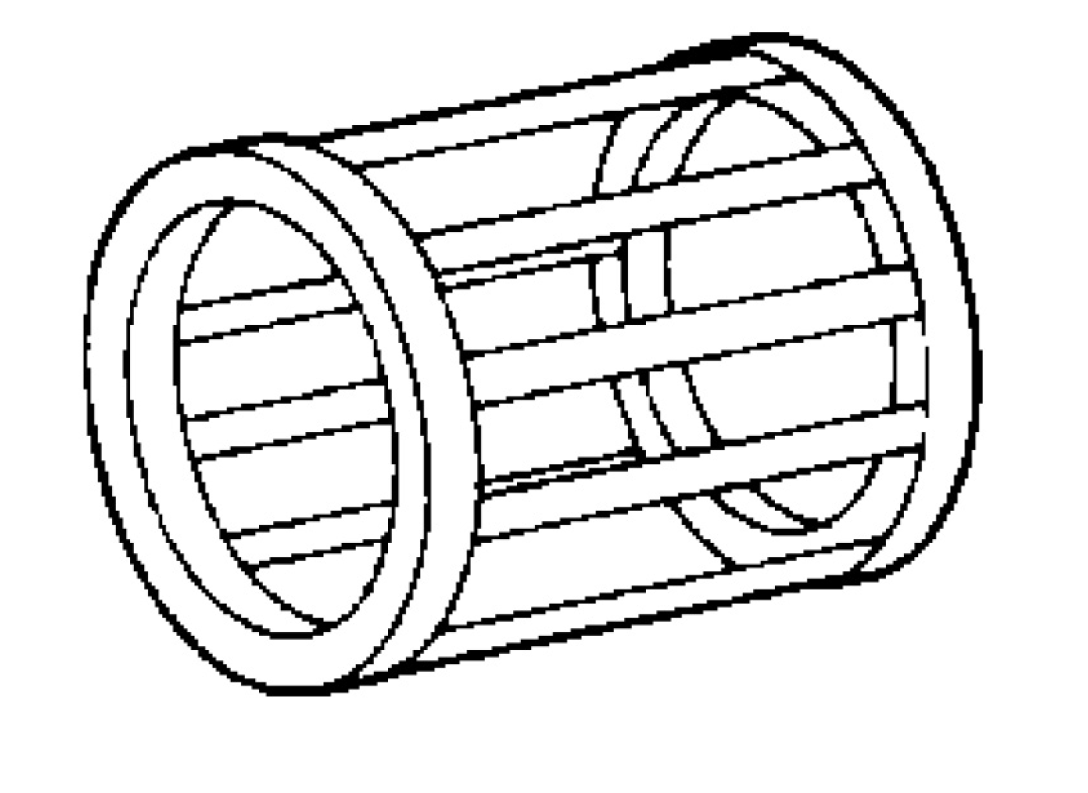
\includegraphics[width=0.3 \textwidth]{./img/cage}
}
\begin{solution}
Il s'agit d'un rotor à cage. C'est très courant dans l'industrie car peu cher même si moins pratique que le rotor bobiné triphasé.\\
Sans surprise l'autre type de machine asynchrone est donc la machine à rotor bobiné !
\end{solution}

\end{questions}



\blfootnote{La dernière version de ce document au format PDF est disponible à l'adresse suivante: \url{https://github.com/rmelotte/electricite/blob/master/main.pdf}\\
Si vous souhaitez y apporter des modifications, trois possibilités s'offrent à vous: vous pouvez le modifier directement en ligne à l'adresse suivante: \url{https://www.overleaf.com/5344493hybftn}, si vous avez déjà utilisé la platforme GitHub, le document est aussi accessible ici: \url{https://github.com/rmelotte/electricite}. Enfin, vous pouvez aussi envoyer vos modifications par email, à l'adresse suivante: \href{mailto:raphael.melotte@gmail.com}{raphael.melotte@gmail.com}. Toute contribution est la bienvenue!}

\end{document}